\documentclass{beamer}
\usetheme{metropolis}
\usepackage{../../resources/style}
\usepackage{colortbl}
\usetikzlibrary{matrix}

\newcommand{\beginnote}[1]{%
  \vfill
  {\footnotesize\textcolor{gray}{\textit{$\triangleright$ #1 (vezi slide-ul \emph{Resurse})}}}%
}

\title{Sume parțiale \textbar\ Șmenul lui Mars}
\subtitle{Tablouri unidimensionale $\cdot$ Tablouri bidimensionale}
\author{Andrei Mihai Ciobanu}
\institute{Algolymp Summer School}
\date{}
\titlegraphic{
\includegraphics[width=4cm]{../../resources/algolymp-logo.png}}
\setbeamertemplate{frame footer}{Algolymp Summer School}

% ----------------------------------------------------------------
\begin{document}

\begin{frame}[shrink]
  \titlepage
\end{frame}

\begin{frame}{Cuprins}
  \tableofcontents
\end{frame}

% ================================================================
\section{Sume parțiale pe vectori}

\begin{frame}{Problema}
  Avem un vector $a[1 \ldots n]$ și $Q$ interogări de tipul:
  \begin{block}{Interogare}
    Care este suma $a[l] + a[l+1] + \ldots + a[r]$?
  \end{block}

  \smallskip
  \textbf{Soluție naivă}: parcurgem elementele din $[l, r]$ și le adunăm.
  \begin{itemize}
    \item O interogare costă $O(n)$ \textemdash{} $Q$ interogări costă $O(n \cdot Q)$
    \item Pentru $n = Q = 10^5$: $10^{10}$ operații \textemdash{} prea lent!
  \end{itemize}

  \smallskip
  \textbf{Idee}: facem o precalculare în $O(n)$ care ne permite să răspundem la fiecare interogare în $O(1)$.

  \begin{center}
  \begin{tabular}{lcc}
    \toprule
    Abordare & Precalcul & Per interogare \\
    \midrule
    Naivă         & $O(1)$    & $O(n)$ \\
    Sume parțiale & $O(n)$    & $O(1)$ \\
    \bottomrule
  \end{tabular}
  \end{center}
\end{frame}

\begin{frame}{Ce stochează $S[i]$?}
  Construim un vector auxiliar $S[0 \ldots n]$ cu proprietatea:

  $S[i]$ = suma primelor $i$ elemente din $a$\quad ($S[0] = 0$ prin convenție)

  \textbf{Exemplu} cu $a = [3,\ 1,\ 4,\ 1,\ 5,\ 9]$:

  \begin{center}
  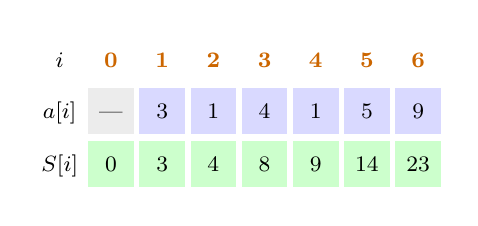
\begin{tikzpicture}
  \matrix[matrix of nodes, nodes in empty cells, ampersand replacement=\&,
          nodes={minimum size=0.58cm, text width=0.58cm, inner sep=0pt,
                 align=center, font=\footnotesize, execute at begin node={\vphantom{0}}},
          row sep=2pt, column sep=2pt] {
    |[font=\footnotesize\bfseries]| $i$
      \& |[font=\footnotesize\bfseries, text=orange!80!black]| 0
      \& |[font=\footnotesize\bfseries, text=orange!80!black]| 1
      \& |[font=\footnotesize\bfseries, text=orange!80!black]| 2
      \& |[font=\footnotesize\bfseries, text=orange!80!black]| 3
      \& |[font=\footnotesize\bfseries, text=orange!80!black]| 4
      \& |[font=\footnotesize\bfseries, text=orange!80!black]| 5
      \& |[font=\footnotesize\bfseries, text=orange!80!black]| 6 \\
    |[font=\footnotesize\bfseries]| $a[i]$
      \& |[fill=gray!15]| \textemdash{}
      \& |[fill=blue!15]| 3 \& |[fill=blue!15]| 1
      \& |[fill=blue!15]| 4 \& |[fill=blue!15]| 1
      \& |[fill=blue!15]| 5 \& |[fill=blue!15]| 9 \\
    |[font=\footnotesize\bfseries]| $S[i]$
      \& |[fill=green!20]| 0
      \& |[fill=green!20]| 3 \& |[fill=green!20]| 4
      \& |[fill=green!20]| 8 \& |[fill=green!20]| 9
      \& |[fill=green!20]| 14 \& |[fill=green!20]| 23 \\
  };
  \end{tikzpicture}
  \end{center}

  \smallskip
  $S[3] = a[1]+a[2]+a[3] = 3+1+4 = 8$ \hfill
  $S[5] = a[1]+\ldots+a[5] = 14$

  \smallskip
  \textbf{Construcție:} pornim cu $S[0]=0$, apoi $S[i] = S[i-1] + a[i]$
\end{frame}

\begin{frame}[shrink]{Cum aflăm suma unui segment?}
  \textbf{Interogare:} $\mathrm{sum}(l, r) = S[r] - S[l-1]$

  \textbf{De ce funcționează?} Scriem explicit ce conține fiecare termen:
  \begin{align*}
    S[r]   &= a[1] + a[2] + \ldots + a[l-1] + a[l] + \ldots + a[r] \\
    S[l-1] &= a[1] + a[2] + \ldots + a[l-1]
  \end{align*}
  \[
    S[r] - S[l-1] = a[l] + a[l+1] + \ldots + a[r] \quad \checkmark
  \]

  \smallskip
  \textbf{Exemplu}: $\mathrm{sum}(3, 5)$ pe $a = [3,1,4,1,5,9]$:

  \begin{center}
  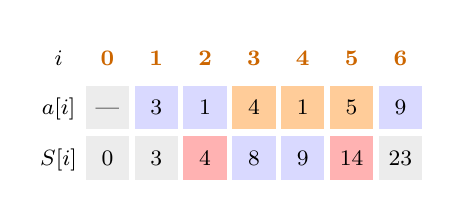
\begin{tikzpicture}
  \matrix[matrix of nodes, nodes in empty cells, ampersand replacement=\&,
          nodes={minimum size=0.55cm, text width=0.55cm, inner sep=0pt,
                 align=center, font=\footnotesize, execute at begin node={\vphantom{0}}},
          row sep=2pt, column sep=2pt] {
    |[font=\footnotesize\bfseries]| $i$
      \& |[font=\footnotesize\bfseries, text=orange!80!black]| 0
      \& |[font=\footnotesize\bfseries, text=orange!80!black]| 1
      \& |[font=\footnotesize\bfseries, text=orange!80!black]| 2
      \& |[font=\footnotesize\bfseries, text=orange!80!black]| 3
      \& |[font=\footnotesize\bfseries, text=orange!80!black]| 4
      \& |[font=\footnotesize\bfseries, text=orange!80!black]| 5
      \& |[font=\footnotesize\bfseries, text=orange!80!black]| 6 \\
    |[font=\footnotesize\bfseries]| $a[i]$
      \& |[fill=gray!15]| \textemdash{}
      \& |[fill=blue!15]| 3 \& |[fill=blue!15]| 1
      \& |[fill=orange!40]| 4 \& |[fill=orange!40]| 1 \& |[fill=orange!40]| 5
      \& |[fill=blue!15]| 9 \\
    |[font=\footnotesize\bfseries]| $S[i]$
      \& |[fill=gray!15]| 0
      \& |[fill=gray!15]| 3 \& |[fill=red!30]| 4
      \& |[fill=blue!15]| 8 \& |[fill=blue!15]| 9 \& |[fill=red!30]| 14
      \& |[fill=gray!15]| 23 \\
  };
  \end{tikzpicture}
  \end{center}

  $\mathrm{sum}(3,5) = S[5] - S[2] = 14 - 4 = 10 \quad (4+1+5=10\ \checkmark)$
\end{frame}

\begin{frame}[fragile, shrink]{Implementare}
  \begin{lstlisting}
const int nmax = 100000;
int a[nmax + 1];
long long S[nmax + 1];
int n, q, l, r;

// precalcul: O(n)
// S[0] = 0 automat (declarare globala)
for (int i = 1; i <= n; i++) {
    S[i] = S[i - 1] + a[i];
}

// interogare sum(l, r): O(1)
long long suma = S[r] - S[l - 1];
  \end{lstlisting}

  \begin{itemize}
    \item \alert{Atenție la overflow!} Dacă $a[i]$ pot fi mari, $S[i]$ poate depăși \texttt{int}
  \end{itemize}
\end{frame}

% ================================================================
\section{Sume parțiale pe matrici}

\begin{frame}{De la 1D la 2D}
  Aceeași idee, extinsă la matrici; definim:

  $S[i][j]$ = suma tuturor elementelor din submatricea cu colțul stânga-sus la $(1,1)$ și colțul dreapta-jos la $(i,j)$

  \vfill

  \begin{columns}[c]
    \column{0.50\textwidth}
    \begin{center}
    \textbf{Matricea $a$:}

    \smallskip
    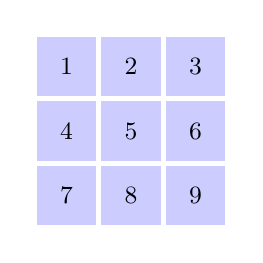
\begin{tikzpicture}
    \matrix[matrix of nodes, nodes in empty cells, ampersand replacement=\&,
            nodes={minimum size=0.75cm, text width=0.75cm, inner sep=0pt,
                   align=center, font=\small, execute at begin node={\vphantom{0}}},
            row sep=2pt, column sep=2pt] {
      |[fill=blue!20]| 1 \& |[fill=blue!20]| 2 \& |[fill=blue!20]| 3 \\
      |[fill=blue!20]| 4 \& |[fill=blue!20]| 5 \& |[fill=blue!20]| 6 \\
      |[fill=blue!20]| 7 \& |[fill=blue!20]| 8 \& |[fill=blue!20]| 9 \\
    };
    \end{tikzpicture}
    \end{center}

    \column{0.50\textwidth}
    \begin{center}
    \textbf{Matricea $S$:}

    \smallskip
    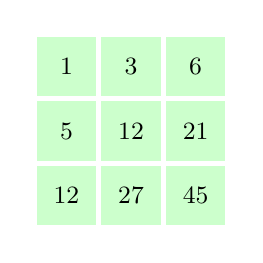
\begin{tikzpicture}
    \matrix[matrix of nodes, nodes in empty cells, ampersand replacement=\&,
            nodes={minimum size=0.75cm, text width=0.75cm, inner sep=0pt,
                   align=center, font=\small, execute at begin node={\vphantom{0}}},
            row sep=2pt, column sep=2pt] {
      |[fill=green!20]| 1 \& |[fill=green!20]| 3 \& |[fill=green!20]| 6 \\
      |[fill=green!20]| 5 \& |[fill=green!20]| 12 \& |[fill=green!20]| 21 \\
      |[fill=green!20]| 12 \& |[fill=green!20]| 27 \& |[fill=green!20]| 45 \\
    };
    \end{tikzpicture}
    \end{center}
  \end{columns}

  \vfill

  \begin{center}
    $S[2][3] = 1+2+3+4+5+6 = 21$ \qquad $S[3][3] = 1+2+\ldots+9 = 45$
  \end{center}
\end{frame}

\begin{frame}[shrink]{Construcție}
  Calculăm $S$ rând cu rând, coloană cu coloană. La momentul calculului lui $S[i][j]$, valorile de deasupra și din stânga sunt deja cunoscute:

  \smallskip
  \textbf{Ce avem calculat în jurul lui $S[i][j]$?}
  \begin{itemize}
    \item $S[i{-}1][j]$ \textemdash{} suma dreptunghiului de deasupra
    \item $S[i][j{-}1]$ \textemdash{} suma dreptunghiului din stânga
    \item $S[i{-}1][j{-}1]$ \textemdash{} suma dreptunghiului din colțul stânga-sus
  \end{itemize}

  \smallskip
  \textbf{Cum calculăm $S[i][j]$?}
  \begin{itemize}
    \item Adunăm $S[i{-}1][j]$ și $S[i][j{-}1]$ \textemdash{} zona deasupra + zona din stânga
    \item $S[i{-}1][j{-}1]$ a fost adăugat de două ori $\Rightarrow$ îl scădem
    \item Adăugăm $a[i][j]$ \textemdash{} celula curentă
  \end{itemize}

  \[S[i][j] = S[i{-}1][j] + S[i][j{-}1] - S[i{-}1][j{-}1] + a[i][j]\]
\end{frame}

\begin{frame}{De ce funcționează formula?}
  Exemplu: calculul lui $S[3][3]$ pe o matrice $3\times3$. Numerele arată de câte ori a fost adăugată fiecare celulă:

  \smallskip
  \begin{columns}[c]
    \column{0.25\textwidth}
    \centering
    {\footnotesize $+S[2][3]$}
    \begin{center}
    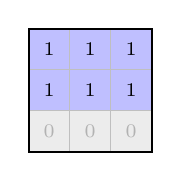
\begin{tikzpicture}[scale=0.52]
      \fill[blue!25] (0,1) rectangle (3,3);
      \fill[gray!15] (0,0) rectangle (3,1);
      \draw[gray!50, very thin] (0,0) grid (3,3);
      \draw[thick] (0,0) rectangle (3,3);
      \node[font=\scriptsize] at (0.5,2.5) {1}; \node[font=\scriptsize] at (1.5,2.5) {1}; \node[font=\scriptsize] at (2.5,2.5) {1};
      \node[font=\scriptsize] at (0.5,1.5) {1}; \node[font=\scriptsize] at (1.5,1.5) {1}; \node[font=\scriptsize] at (2.5,1.5) {1};
      \node[font=\scriptsize,text=gray!60] at (0.5,0.5) {0}; \node[font=\scriptsize,text=gray!60] at (1.5,0.5) {0}; \node[font=\scriptsize,text=gray!60] at (2.5,0.5) {0};
    \end{tikzpicture}
    \end{center}

    \column{0.25\textwidth}
    \centering
    {\footnotesize $+S[3][2]$}
    \begin{center}
    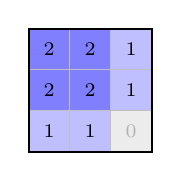
\begin{tikzpicture}[scale=0.52]
      \fill[blue!50] (0,1) rectangle (2,3);
      \fill[blue!25] (2,1) rectangle (3,3);
      \fill[blue!25] (0,0) rectangle (2,1);
      \fill[gray!15] (2,0) rectangle (3,1);
      \draw[gray!50, very thin] (0,0) grid (3,3);
      \draw[thick] (0,0) rectangle (3,3);
      \node[font=\scriptsize] at (0.5,2.5) {2}; \node[font=\scriptsize] at (1.5,2.5) {2}; \node[font=\scriptsize] at (2.5,2.5) {1};
      \node[font=\scriptsize] at (0.5,1.5) {2}; \node[font=\scriptsize] at (1.5,1.5) {2}; \node[font=\scriptsize] at (2.5,1.5) {1};
      \node[font=\scriptsize] at (0.5,0.5) {1}; \node[font=\scriptsize] at (1.5,0.5) {1}; \node[font=\scriptsize,text=gray!60] at (2.5,0.5) {0};
    \end{tikzpicture}
    \end{center}

    \column{0.25\textwidth}
    \centering
    {\footnotesize $-S[2][2]$}
    \begin{center}
    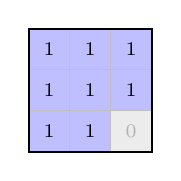
\begin{tikzpicture}[scale=0.52]
      \fill[blue!25] (0,0) rectangle (3,3);
      \fill[gray!15] (2,0) rectangle (3,1);
      \draw[gray!50, very thin] (0,0) grid (3,3);
      \draw[thick] (0,0) rectangle (3,3);
      \node[font=\scriptsize] at (0.5,2.5) {1}; \node[font=\scriptsize] at (1.5,2.5) {1}; \node[font=\scriptsize] at (2.5,2.5) {1};
      \node[font=\scriptsize] at (0.5,1.5) {1}; \node[font=\scriptsize] at (1.5,1.5) {1}; \node[font=\scriptsize] at (2.5,1.5) {1};
      \node[font=\scriptsize] at (0.5,0.5) {1}; \node[font=\scriptsize] at (1.5,0.5) {1}; \node[font=\scriptsize,text=gray!60] at (2.5,0.5) {0};
    \end{tikzpicture}
    \end{center}

    \column{0.25\textwidth}
    \centering
    {\footnotesize $+a[3][3]$}
    \begin{center}
    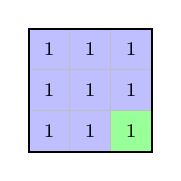
\begin{tikzpicture}[scale=0.52]
      \fill[blue!25] (0,0) rectangle (3,3);
      \fill[green!40] (2,0) rectangle (3,1);
      \draw[gray!50, very thin] (0,0) grid (3,3);
      \draw[thick] (0,0) rectangle (3,3);
      \node[font=\scriptsize] at (0.5,2.5) {1}; \node[font=\scriptsize] at (1.5,2.5) {1}; \node[font=\scriptsize] at (2.5,2.5) {1};
      \node[font=\scriptsize] at (0.5,1.5) {1}; \node[font=\scriptsize] at (1.5,1.5) {1}; \node[font=\scriptsize] at (2.5,1.5) {1};
      \node[font=\scriptsize] at (0.5,0.5) {1}; \node[font=\scriptsize] at (1.5,0.5) {1}; \node[font=\scriptsize] at (2.5,0.5) {1};
    \end{tikzpicture}
    \end{center}
  \end{columns}

  \vfill
  \begin{center}
    \small Fiecare celulă apare exact o dată $\Rightarrow$ $S[3][3]$ = suma celor 9 elemente \checkmark
  \end{center}
\end{frame}

\begin{frame}[shrink]{Interogarea}
  Vrem suma elementelor din submatricea cu colțul stânga-sus $(r_1,c_1)$ și dreapta-jos $(r_2,c_2)$:

  \smallskip
  \textbf{Cum?} Construim răspunsul din valorile lui $S$ deja calculate:
  \begin{itemize}
    \item Pornim cu $S[r_2][c_2]$ \textemdash{} include tot de la $(1,1)$ la $(r_2,c_2)$
    \item Scădem $S[r_1{-}1][c_2]$ \textemdash{} eliminăm banda de deasupra zonei dorite
    \item Scădem $S[r_2][c_1{-}1]$ \textemdash{} eliminăm banda din stânga zonei dorite
    \item Adunăm $S[r_1{-}1][c_1{-}1]$ \textemdash{} colțul stânga-sus a fost scăzut de două ori, îl readăugăm
  \end{itemize}

  \begin{align*}
    \mathrm{sum}(r_1,c_1,r_2,c_2) = {}&S[r_2][c_2] - S[r_1{-}1][c_2]\\
    &- S[r_2][c_1{-}1] + S[r_1{-}1][c_1{-}1]
  \end{align*}
\end{frame}

\begin{frame}{De ce funcționează interogarea?}
  Exemplu: suma submatricei $(2,2)\ldots(4,4)$ pe o matrice $4\times4$:

  \smallskip
  \begin{columns}[c]
    \column{0.25\textwidth}
    \centering
    {\footnotesize $+S[4][4]$}
    \begin{center}
    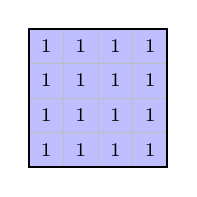
\begin{tikzpicture}[scale=0.44]
      \fill[blue!25] (0,0) rectangle (4,4);
      \draw[gray!50, very thin] (0,0) grid (4,4);
      \draw[thick] (0,0) rectangle (4,4);
      \foreach \r in {0,1,2,3} {
        \foreach \c in {0,1,2,3} {
          \node[font=\scriptsize] at (\c+0.5,\r+0.5) {1};
        }
      }
    \end{tikzpicture}
    \end{center}

    \column{0.25\textwidth}
    \centering
    {\footnotesize $-S[1][4]$}
    \begin{center}
    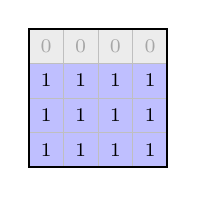
\begin{tikzpicture}[scale=0.44]
      \fill[blue!25] (0,0) rectangle (4,3);
      \fill[gray!15] (0,3) rectangle (4,4);
      \draw[gray!50, very thin] (0,0) grid (4,4);
      \draw[thick] (0,0) rectangle (4,4);
      \foreach \c in {0,1,2,3} {
        \node[font=\scriptsize,text=gray!70] at (\c+0.5,3.5) {0};
      }
      \foreach \r in {0,1,2} {
        \foreach \c in {0,1,2,3} {
          \node[font=\scriptsize] at (\c+0.5,\r+0.5) {1};
        }
      }
    \end{tikzpicture}
    \end{center}

    \column{0.25\textwidth}
    \centering
    {\footnotesize $-S[4][1]$}
    \begin{center}
    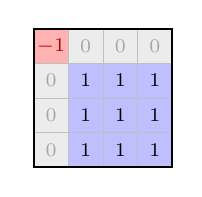
\begin{tikzpicture}[scale=0.44]
      \fill[gray!15] (0,0) rectangle (4,4);
      \fill[blue!25] (1,0) rectangle (4,3);
      \fill[red!30]  (0,3) rectangle (1,4);
      \draw[gray!50, very thin] (0,0) grid (4,4);
      \draw[thick] (0,0) rectangle (4,4);
      \node[font=\scriptsize,text=red!70!black] at (0.5,3.5) {$-1$};
      \foreach \c in {1,2,3} { \node[font=\scriptsize,text=gray!70] at (\c+0.5,3.5) {0}; }
      \foreach \r in {0,1,2} { \node[font=\scriptsize,text=gray!70] at (0.5,\r+0.5) {0}; }
      \foreach \r in {0,1,2} {
        \foreach \c in {1,2,3} {
          \node[font=\scriptsize] at (\c+0.5,\r+0.5) {1};
        }
      }
    \end{tikzpicture}
    \end{center}

    \column{0.25\textwidth}
    \centering
    {\footnotesize $+S[1][1]$}
    \begin{center}
    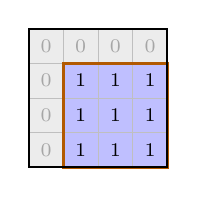
\begin{tikzpicture}[scale=0.44]
      \fill[gray!15] (0,0) rectangle (4,4);
      \fill[blue!25] (1,0) rectangle (4,3);
      \draw[gray!50, very thin] (0,0) grid (4,4);
      \draw[thick, orange!70!black, line width=1.2pt] (1,0) rectangle (4,3);
      \draw[thick] (0,0) rectangle (4,4);
      \foreach \c in {0,1,2,3} { \node[font=\scriptsize,text=gray!70] at (\c+0.5,3.5) {0}; }
      \foreach \r in {0,1,2} { \node[font=\scriptsize,text=gray!70] at (0.5,\r+0.5) {0}; }
      \foreach \r in {0,1,2} {
        \foreach \c in {1,2,3} {
          \node[font=\scriptsize] at (\c+0.5,\r+0.5) {1};
        }
      }
    \end{tikzpicture}
    \end{center}
  \end{columns}

  \vfill
  \begin{center}
    \small Zona $(2,2)\ldots(4,4)$ — toate celulele cu valoarea 1 $\Rightarrow$ suma corectă \checkmark
  \end{center}
\end{frame}

\begin{frame}[fragile, shrink]{Implementare}
  \begin{lstlisting}
const int nmax = 1000;
int a[nmax + 1][nmax + 1];
long long S[nmax + 1][nmax + 1];

// precalculare: O(n * m)
for (int i = 1; i <= n; i++) {
    for (int j = 1; j <= m; j++) {
        S[i][j] = S[i - 1][j] + S[i][j - 1]
                  - S[i-1][j-1] + a[i][j];
    }
}

// interogare (r1,c1)..(r2,c2): O(1)
long long suma = S[r2][c2] - S[r1 - 1][c2]
                 - S[r2][c1 - 1] + S[r1 - 1][c1 - 1];
  \end{lstlisting}

  \begin{itemize}
    \item \alert{Atenție:} de cele mai multe ori suma valorilor matricii poate deveni foarte mare, în consecință declarăm $S$ ca \texttt{long long}
  \end{itemize}
\end{frame}

% ================================================================
\section{Șmenul lui Mars pe vector}

\begin{frame}[shrink]{Problema}
  Avem un vector $a[1 \ldots n]$ și $Q$ operații:
  \begin{block}{Update}
    Adaugă valoarea $v$ la toate elementele $a[l], \ldots, a[r]$
  \end{block}

  \smallskip
  \begin{itemize}
    \item \textbf{Soluție naivă}: parcurgem $[l, r]$ și adăugăm $v$ \textemdash{} $O(n)$ per update
    \item \textbf{Șmenul lui Mars}: fiecare update în $O(1)$, reconstituire finală în $O(n)$
  \end{itemize}

  \smallskip
  \begin{center}
  \begin{tabular}{lcc}
    \toprule
    Tehnică & Update pe interval & Citire element \\
    \midrule
    Naiv & $O(n)$ & $O(1)$ \\
    Șmenul lui Mars & $O(1)$ & $O(n)$ reconstituire \\
    \bottomrule
  \end{tabular}
  \end{center}
  \medskip
  Optim când facem \textbf{toate update-urile mai întâi}, apoi citim rezultatul.
\end{frame}

\begin{frame}{Vectorul de diferențe}
  \begin{block}{Definiție}
    $D[i] = a[i] - a[i-1]$, cu $a[0] = 0$
  \end{block}

  \textbf{Update $[l, r]$ cu $+v$:} doar două operații!
  \begin{itemize}
    \item $D[l] \mathrel{+}= v$
    \item $D[r+1] \mathrel{-}= v$
  \end{itemize}

  \smallskip
  \textbf{Exemplu:} adăugăm $+3$ pe $[2, 4]$ în $a = [0,0,0,0,0]$:

  \begin{center}
  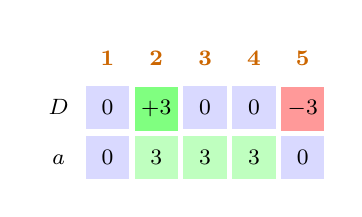
\begin{tikzpicture}
  \matrix[matrix of nodes, nodes in empty cells, ampersand replacement=\&,
          nodes={minimum size=0.55cm, text width=0.55cm, inner sep=0pt,
                 align=center, font=\footnotesize, execute at begin node={\vphantom{0}}},
          row sep=2pt, column sep=2pt] {
    {} \& |[font=\footnotesize\bfseries, text=orange!80!black]| 1
       \& |[font=\footnotesize\bfseries, text=orange!80!black]| 2
       \& |[font=\footnotesize\bfseries, text=orange!80!black]| 3
       \& |[font=\footnotesize\bfseries, text=orange!80!black]| 4
       \& |[font=\footnotesize\bfseries, text=orange!80!black]| 5 \\
    |[font=\footnotesize\bfseries]| $D$
       \& |[fill=blue!15]| 0 \& |[fill=green!50]| $+3$
       \& |[fill=blue!15]| 0 \& |[fill=blue!15]| 0 \& |[fill=red!40]| $-3$ \\
    |[font=\footnotesize\bfseries]| $a$
       \& |[fill=blue!15]| 0 \& |[fill=green!25]| 3
       \& |[fill=green!25]| 3 \& |[fill=green!25]| 3 \& |[fill=blue!15]| 0 \\
  };
  \end{tikzpicture}
  \end{center}

  \textbf{Observație:} $D$ e vectorul de diferențe al lui $a$ $\Longleftrightarrow$ prin sume parțiale pe $D$ obținem $a$
\end{frame}

\begin{frame}[fragile]{Implementare}
  \begin{lstlisting}
const int nmax = 100000;
int D[nmax + 2]; // vectorul de diferente
int n, q;

// update [l, r] cu +v: O(1)
D[l] += v;
D[r + 1] -= v;

// reconstruire finala: O(n)
for (int i = 1; i <= n; i++) {
    D[i] += D[i - 1]; // D[i] devine a[i]
}
  \end{lstlisting}

  \begin{itemize}
    \item $D$ trebuie dimensionat cu $n+1$ pentru a evita depășirea la $D[r+1]$
    \item Reconstituirea se face o singură dată, \textbf{după} toate update-urile
  \end{itemize}
\end{frame}

% ================================================================
\section{Șmenul lui Mars pe matrici}

\begin{frame}{Extensia la matrici}
  \textbf{Update pe submatricea $(r_1,c_1)\ldots(r_2,c_2)$ cu $+v$} \textemdash{} 4 modificări în colțuri:

  \begin{columns}[T]
    \column{0.52\textwidth}
    \begin{block}{Cele 4 actualizări}
      \begin{itemize}\itemsep3pt
        \item $D[r_1][c_1] \mathrel{+}= v$
        \item $D[r_1][c_2{+}1] \mathrel{-}= v$
        \item $D[r_2{+}1][c_1] \mathrel{-}= v$
        \item $D[r_2{+}1][c_2{+}1] \mathrel{+}= v$
      \end{itemize}
    \end{block}

    \smallskip
    \textbf{Reconstituire:} sumă parțială 2D aplicată pe $D$ (aceeași formulă ca la sume parțiale 2D).

    \column{0.42\textwidth}
    \begin{center}
    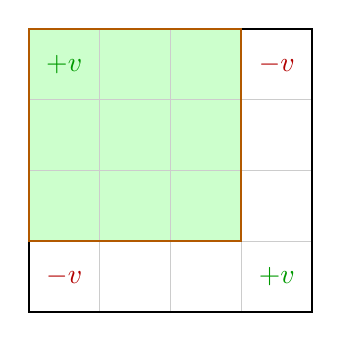
\begin{tikzpicture}[scale=0.9]
      \fill[green!20] (0,1) rectangle (3,4);
      \draw[gray!40, very thin] (0,0) grid (4,4);
      \draw[thick] (0,0) rectangle (4,4);
      \draw[thick, orange!70!black] (0,1) rectangle (3,4);
      \node[font=\small, text=green!60!black, font=\bfseries] at (0.5,3.5) {$+v$};
      \node[font=\small, text=red!70!black,   font=\bfseries] at (3.5,3.5) {$-v$};
      \node[font=\small, text=red!70!black,   font=\bfseries] at (0.5,0.5) {$-v$};
      \node[font=\small, text=green!60!black, font=\bfseries] at (3.5,0.5) {$+v$};
    \end{tikzpicture}
    \end{center}
  \end{columns}
\end{frame}

\begin{frame}[shrink]{De ce funcționează?}
  Exemplu: $+3$ pe $(2,2)\ldots(3,3)$ în matricea $4{\times}4$ zero.
  Urmărim $D$ și $a$ reconstituită după fiecare colț adăugat:

  \begin{columns}[T]

    % ---- Op 1: D[2][2] += 3 ----
    \column{0.25\textwidth}
    \begin{center}
    {\footnotesize $D[2][2]\mathrel{+}=3$}

    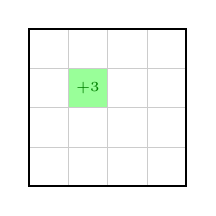
\begin{tikzpicture}[scale=0.5]
      \fill[green!40] (1,2) rectangle (2,3);
      \draw[gray!40, very thin] (0,0) grid (4,4);
      \draw[thick] (0,0) rectangle (4,4);
      \node[font=\tiny\bfseries, text=green!50!black] at (1.5,2.5) {$+3$};
    \end{tikzpicture}

    \smallskip
    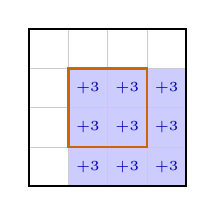
\begin{tikzpicture}[scale=0.5]
      \foreach \r in {2,3,4} {
        \foreach \c in {2,3,4} {
          \fill[blue!20] (\c-1,4-\r) rectangle (\c,5-\r);
          \node[font=\tiny, text=blue!70!black] at (\c-0.5,4.5-\r) {$+3$};
        }
      }
      \draw[gray!40, very thin] (0,0) grid (4,4);
      \draw[thick] (0,0) rectangle (4,4);
      \draw[orange!80!black, line width=1pt] (1,1) rectangle (3,3);
    \end{tikzpicture}

    {\footnotesize $a$}
    \end{center}

    % ---- Op 2: D[2][4] -= 3 ----
    \column{0.25\textwidth}
    \begin{center}
    {\footnotesize $D[2][4]\mathrel{-}=3$}

    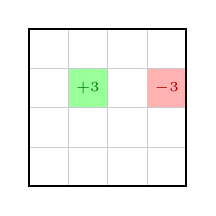
\begin{tikzpicture}[scale=0.5]
      \fill[green!40] (1,2) rectangle (2,3);
      \fill[red!30]   (3,2) rectangle (4,3);
      \draw[gray!40, very thin] (0,0) grid (4,4);
      \draw[thick] (0,0) rectangle (4,4);
      \node[font=\tiny\bfseries, text=green!50!black] at (1.5,2.5) {$+3$};
      \node[font=\tiny\bfseries, text=red!70!black]   at (3.5,2.5) {$-3$};
    \end{tikzpicture}

    \smallskip
    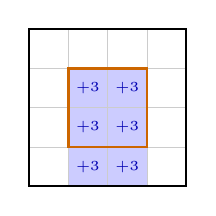
\begin{tikzpicture}[scale=0.5]
      \foreach \r in {2,3,4} {
        \foreach \c in {2,3} {
          \fill[blue!20] (\c-1,4-\r) rectangle (\c,5-\r);
          \node[font=\tiny, text=blue!70!black] at (\c-0.5,4.5-\r) {$+3$};
        }
      }
      \draw[gray!40, very thin] (0,0) grid (4,4);
      \draw[thick] (0,0) rectangle (4,4);
      \draw[orange!80!black, line width=1pt] (1,1) rectangle (3,3);
    \end{tikzpicture}

    {\footnotesize $a$}
    \end{center}

    % ---- Op 3: D[4][2] -= 3 ----
    \column{0.25\textwidth}
    \begin{center}
    {\footnotesize $D[4][2]\mathrel{-}=3$}

    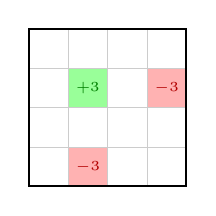
\begin{tikzpicture}[scale=0.5]
      \fill[green!40] (1,2) rectangle (2,3);
      \fill[red!30]   (3,2) rectangle (4,3);
      \fill[red!30]   (1,0) rectangle (2,1);
      \draw[gray!40, very thin] (0,0) grid (4,4);
      \draw[thick] (0,0) rectangle (4,4);
      \node[font=\tiny\bfseries, text=green!50!black] at (1.5,2.5) {$+3$};
      \node[font=\tiny\bfseries, text=red!70!black]   at (3.5,2.5) {$-3$};
      \node[font=\tiny\bfseries, text=red!70!black]   at (1.5,0.5) {$-3$};
    \end{tikzpicture}

    \smallskip
    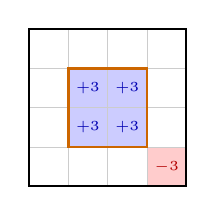
\begin{tikzpicture}[scale=0.5]
      \foreach \r in {2,3} {
        \foreach \c in {2,3} {
          \fill[blue!20] (\c-1,4-\r) rectangle (\c,5-\r);
          \node[font=\tiny, text=blue!70!black] at (\c-0.5,4.5-\r) {$+3$};
        }
      }
      \fill[red!20] (3,0) rectangle (4,1);
      \draw[gray!40, very thin] (0,0) grid (4,4);
      \draw[thick] (0,0) rectangle (4,4);
      \draw[orange!80!black, line width=1pt] (1,1) rectangle (3,3);
      \node[font=\tiny\bfseries, text=red!70!black] at (3.5,0.5) {$-3$};
    \end{tikzpicture}

    {\footnotesize $a$}
    \end{center}

    % ---- Op 4: D[4][4] += 3 ----
    \column{0.25\textwidth}
    \begin{center}
    {\footnotesize $D[4][4]\mathrel{+}=3$}

    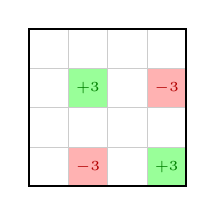
\begin{tikzpicture}[scale=0.5]
      \fill[green!40] (1,2) rectangle (2,3);
      \fill[red!30]   (3,2) rectangle (4,3);
      \fill[red!30]   (1,0) rectangle (2,1);
      \fill[green!40] (3,0) rectangle (4,1);
      \draw[gray!40, very thin] (0,0) grid (4,4);
      \draw[thick] (0,0) rectangle (4,4);
      \node[font=\tiny\bfseries, text=green!50!black] at (1.5,2.5) {$+3$};
      \node[font=\tiny\bfseries, text=red!70!black]   at (3.5,2.5) {$-3$};
      \node[font=\tiny\bfseries, text=red!70!black]   at (1.5,0.5) {$-3$};
      \node[font=\tiny\bfseries, text=green!50!black] at (3.5,0.5) {$+3$};
    \end{tikzpicture}

    \smallskip
    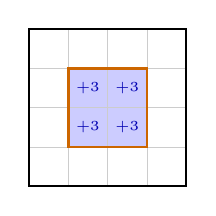
\begin{tikzpicture}[scale=0.5]
      \foreach \r in {2,3} {
        \foreach \c in {2,3} {
          \fill[blue!20] (\c-1,4-\r) rectangle (\c,5-\r);
          \node[font=\tiny, text=blue!70!black] at (\c-0.5,4.5-\r) {$+3$};
        }
      }
      \draw[gray!40, very thin] (0,0) grid (4,4);
      \draw[thick] (0,0) rectangle (4,4);
      \draw[orange!80!black, line width=1pt] (1,1) rectangle (3,3);
    \end{tikzpicture}

    {\footnotesize $a$}
    \end{center}

  \end{columns}
\end{frame}

\begin{frame}[fragile, shrink]{Implementare}
  \begin{lstlisting}
const int nmax = 1000;
long long D[nmax + 2][nmax + 2];

// update (r1,c1)..(r2,c2) cu +v: O(1)
void update(int r1, int c1, int r2, int c2,
            long long v) {
    D[r1][c1] += v;
    D[r1][c2 + 1] -= v;
    D[r2 + 1][c1] -= v;
    D[r2 + 1][c2 + 1] += v;
}

// reconstituire finala: O(n*m)
for (int i = 1; i <= n; i++) {
    for (int j = 1; j <= m; j++) {
        D[i][j] += D[i-1][j] + D[i][j-1] - D[i-1][j-1];
    }
}
  \end{lstlisting}
\end{frame}

% ================================================================
\section{Recapitulare}

\begin{frame}{Recapitulare}
  \begin{center}
  \begin{tabular}{lccc}
    \toprule
    Tehnică & Precalcul & Interogare & Update interval \\
    \midrule
    Sume parțiale 1D   & $O(n)$    & $O(1)$    & $O(n)$ \\
    Sume parțiale 2D   & $O(nm)$   & $O(1)$    & $O(nm)$ \\
    Șmenul lui Mars 1D & $O(n)$    & $O(n)$    & $O(1)$ \\
    Șmenul lui Mars 2D & $O(nm)$   & $O(nm)$   & $O(1)$ \\
    \bottomrule
  \end{tabular}
  \end{center}

  \smallskip
  \begin{itemize}
    \item \textbf{Sume parțiale}: multe interogări, vectorul nu se modifică
    \item \textbf{Șmenul lui Mars}: multe update-uri pe intervale, citire o singură dată la final
    \item Cele două tehnici sunt \textbf{inverse} una față de cealaltă
  \end{itemize}
\end{frame}

% ================================================================
\section{Resurse}

\begin{frame}{Resurse}
  \begin{itemize}\itemsep6pt
    \item \href{https://www.pbinfo.ro}{\textbf{pbinfo.ro}} \textemdash{} Sume parțiale (RO)
    \item \href{https://www.pbinfo.ro}{\textbf{pbinfo.ro}} \textemdash{} Șmenul lui Mars (RO)
    \item \href{https://usaco.guide/silver/prefix-sums?lang=cpp}{\textbf{USACO Guide}} \textemdash{} Introduction to Prefix Sums (EN)
    \item \href{https://usaco.guide/silver/more-prefix-sums?lang=cpp}{\textbf{USACO Guide}} \textemdash{} More on Prefix Sums (EN)
  \end{itemize}
\end{frame}

% ================================================================
\section{Probleme de antrenament}

\begin{frame}{Probleme de antrenament — Sume parțiale}
  \begin{block}{1D}
    \begin{itemize}\footnotesize\itemsep0pt
      \item \href{https://code.algolymp.com/problems/4203}{\textbf{Constant-Time Range Sums}} \textcolor{gray}{(AlgoCode \#4203)}
      \item \href{https://code.algolymp.com/problems/1835}{\textbf{expresie}} \textcolor{gray}{(AlgoCode \#1835 $\cdot$ OJI 2009 IX)}
      \item \href{https://code.algolymp.com/problems/1866}{\textbf{dominant}} \textcolor{gray}{(AlgoCode \#1866 $\cdot$ OJI 2015 VIII)}
      \item \href{https://code.algolymp.com/problems/2984}{\textbf{Macarie}} \textcolor{gray}{(AlgoCode \#2984 $\cdot$ OJI 2024 IX)}
    \end{itemize}
  \end{block}
  \vspace{-4pt}
  \begin{block}{2D}
    \begin{itemize}\footnotesize\itemsep0pt
      \item \href{https://code.algolymp.com/problems/4216}{\textbf{Matrix Line and Diagonal Sums}} \textcolor{gray}{(AlgoCode \#4216)}
      \item \href{https://code.algolymp.com/problems/1854}{\textbf{pseudobil}} \textcolor{gray}{(AlgoCode \#1854 $\cdot$ OJI 2014 IX)}
      \item \href{https://code.algolymp.com/problems/1905}{\textbf{deminare}} \textcolor{gray}{(AlgoCode \#1905 $\cdot$ OJI 2019 IX)}
    \end{itemize}
  \end{block}
\end{frame}

\begin{frame}{Probleme de antrenament — Șmenul lui Mars}
  \begin{block}{1D}
    \begin{itemize}\footnotesize\itemsep0pt
      \item \href{https://code.algolymp.com/problems/4340}{\textbf{Difference Array Final Values}} \textcolor{gray}{(AlgoCode \#4340)}
      \item \href{https://code.algolymp.com/problems/2287}{\textbf{tv}} \textcolor{gray}{(AlgoCode \#2287 $\cdot$ ONI 2015 VII)}
    \end{itemize}
  \end{block}
  \vspace{-4pt}
  \begin{block}{2D}
    \begin{itemize}\footnotesize\itemsep0pt
      \item \href{https://code.algolymp.com/problems/4217}{\textbf{Rectangle Paint with Difference Arrays}} \textcolor{gray}{(AlgoCode \#4217)}
      \item \href{https://kilonova.ro/problems/1399}{\textbf{drept}} \textcolor{gray}{(Kilonova \#1399 $\cdot$ ONI 2012 X)}
      \item \href{https://code.algolymp.com/problems/3077}{\textbf{Eras}} \textcolor{gray}{(AlgoCode \#3077 $\cdot$ ONI 2024 IX)}
    \end{itemize}
  \end{block}
\end{frame}

\end{document}
